%\pdfoutput=1
\documentclass[11pt]{article}

\usepackage[table,xcdraw]{xcolor}
% \usepackage{ACL2023}
\usepackage{amsmath}
\usepackage{latexsym}
\usepackage[T1]{fontenc}

\usepackage[utf8]{inputenc}
\usepackage{fancyhdr}
\usepackage{graphicx}
\usepackage{float}
\usepackage{subfig}
\usepackage{booktabs}
\usepackage{url}
\usepackage{comment}


%%%%%%%%%%%%%%%%%%% TITLE AND AUTHORS %%%%%%%%%%%%%%%%%%%

\title{IIC3633 Aplicación de recomendación grupal de juegos de mesa utilizando metadata}

\author{\normalfont 
Eduardo Salinas | 21624453 | \texttt{esalinasbarros@uc.cl} \\
Nicolás Gutiérrez | 20203772 | \texttt{njgutierrez@uc.cl} \\
Alfonso Badilla | 20640854 | \texttt{alfonso.badilla@uc.cl} \\
% comment line below if only 3 team members
%Author 4 | SCIPER 4 | \texttt{author4@epfl.ch} \\
}

%%%%%%%%%%%%%%%%%%% PROPOSAL %%%%%%%%%%%%%%%%%%%

\begin{document}
\maketitle
\newpage

\section{Pivoteo en la idea original del proyecto}

El proyecto originalmente consistía en un sistema recomendador de juegos de mesa, que fuera capaz de hacer recomendaciones en base a imágenes y características descriptivas (metadata). La idea era que el sistema fuera multimodal y que pudiera recibir diferentes formatos de datos de entrada para dar recomendaciones válidas que al usuario le gustaran. 

Nosotros decidimos cambiar la idea original del proyecto por una que consideramos que podría llegar a ser más poderosa y que a nivel básico debería devolver resultados pronto. La nueva idea consiste en un sistema recomendador de juegos de mesa, que sea capaz de hacer recomendaciones para grupos en base a características descriptivas (metadata). La idea es que el sistema sea multimodal y que pueda recibir diferentes formatos de datos de entrada para dar recomendaciones válidas que al grupo de usuarios le gusten.


\section{Progreso en el desarrollo de la solución}

Para esta entrega, nosotros hemos entrenado un recomendador sencillo utilizando el algoritmo de filtrado colaborativo. Para esto, utilizamos el dataset de BoardGameGeek que contiene información sobre juegos de mesa y ratings de usuarios. El dataset contiene 10 archivos diferentes, cada uno con información diferente sobre juegos de mesa. El punto de entrada fue el archivo \texttt{user\_ratings.csv} el cual consiste de 19 millones de filas. Por temas de procesamiento limitado de Google Collab (y más tarde de nuestro computador local), se utilizaron 50.000 filas para el entrenamiento inicial.

% Actualizar esto cuando entrenemos el recomendador que use metadata!!!

\section{Experimentación realizada y evaluación intemredia}
A modo de experimentación se entrenaron 4 modelos de recomendación diferentes: ItemKNN, SVD, MostPopular y Random que luego se usarán como baseline. 
De estos, se utilizó ItemKNN para hacer una recomendación de juegos para grupos utilizando la ponderación utilitaria-aditiva (equivalente al promedio) 
la cual se usará como baseline para esta entrega. Ademas, se integro un modelo de la libreria \texttt{fastFM} para crear un modelo capaz de recibir metadata y dar recomendaciones.
Para este caso particular, se entreno el modelo agregando features a items los cuales consistian en las categorias en las que se clasificaba el item a recomendar. Las features que se utilizaron 
consistian en la categoria del juego y la mecanica de este. Estos valores se convirtieron desde un flag binario a una representación vectorial como embeddings.

\section{Analisis preliminar de los resultados}
El recomendador que utiliza metadata lo comparamos con el de ItemKNN para varios grupos de usuarios de 5 integrantes. Para ellos encontramos los siguientes resultados:

\begin{table}[H]
    \centering
    \begin{tabular}{|c|c|c|c|c|}
        \hline
        \textbf{Modelo} & \textbf{Recall@10} & \textbf{Precision@10} & \textbf{NDCG@10} & \textbf{RMSE} \\ \hline
        ItemKNN & - & 0.000386 & 0.000128 & 7.13 \\ \hline
        fastFM \& metadata & 0.107 & 0.0056 & - & - \\ \hline
    \end{tabular}
    \caption{Resultados preliminares de recomendaciones para grupos}
    \label{tab:resultados_preliminares}
\end{table}

Si bien no todas las metricas estan incluidas, se puede observar que el modelo que utiliza metadata tiene un mejor recall y precision que el modelo basado en itemKNN.

% Reemplazar las tablas cuando tengamos los resultados de los modelos.

\begin{comment}
\begin{itemize}
    \item \texttt{games.csv}: Este archivo contiene 22 atributos sobre los juegos calificados y contiene 22.000 juegos diferentes. Entre los atributos tenemos aspectos como la descripción del juego, que se podrían evaluar usando modelos de lenguaje, el año de publicación (que distribuye como se muestra en la figura \ref{fig:publishYear}), el rating promedio recibido, entre otros.
    \item \texttt{ratings\_distribution.csv}: Contiene el total de ratings en cada juego de mesa. En general estos ratings distribuyen como se ve en la figura \ref{fig:distribucionRatings}.
    \item \texttt{temes.csv}: Contiene las temáticas de cada juego como un flag binario. Las 50 más comunes se pueden ver en el gráfico de la figura \ref{fig:tematicasComunes}.
    \item \texttt{mechanics.csv}: Contiene las mecánicas del juego como un flag binario. Las 50 más comunes se pueden ver en el gráfico de la figura \ref{fig:mecanicasComunes}.
    \item \texttt{subcategories.csv}: Contiene las subcategorías de cada juego en formato flag binario.
    \item \texttt{artists\_reduced.csv}: Contiene la información sobre que artista creo cierto juego en formato flag binario. Solo se consideran artistas con mas de 3 juegos creados.
    \item \texttt{designer\_reduced.csv}: Contiene la información sobre que diseñador diseño cierto juego en formato flag binario. Solo se consideran diseñadores con mas de 3 juegos creados.
    \item \texttt{publishers\_reduced.csv}: Contiene la información de las empresas que venden dichos juegos en formato flag binario. Solo se consideran las empresas que veden mas de 3 juegos.
    
\end{itemize}


\begin{figure}
    \centering
    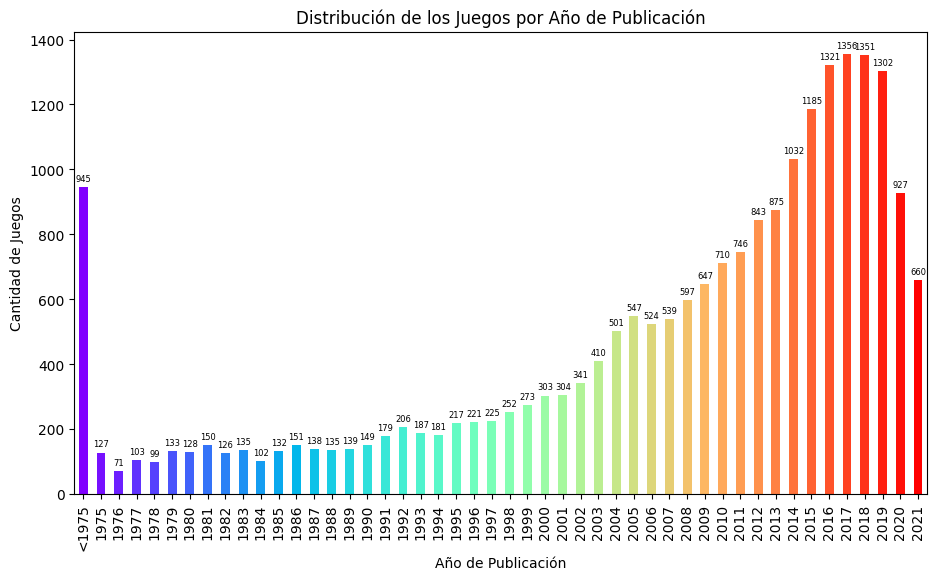
\includegraphics[width=0.8\linewidth]{publishYear.png}
    \caption{Juegos por año de publicación}
    \label{fig:publishYear}
\end{figure}

\begin{figure}[h]
    \centering
    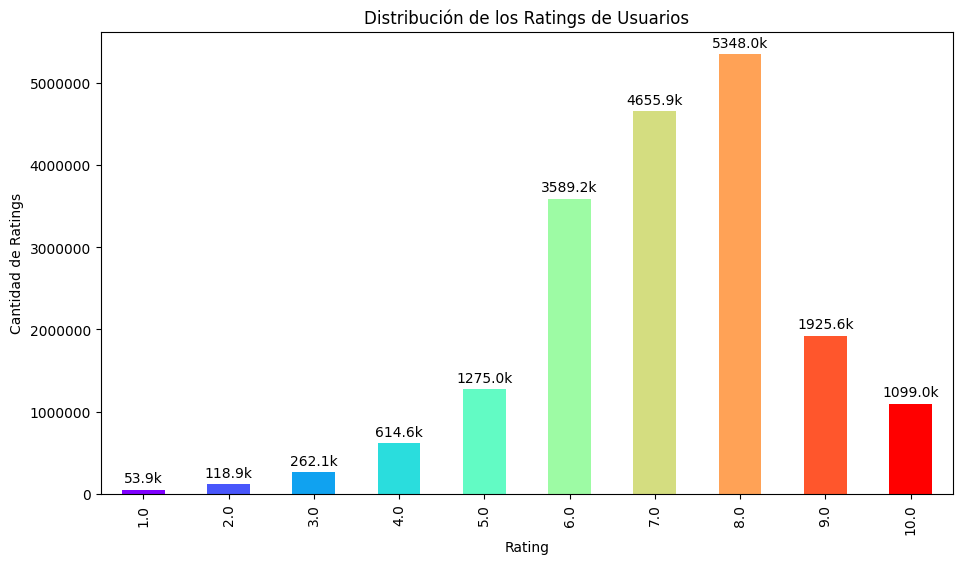
\includegraphics[width=0.8\linewidth]{distribucionRatings.png}
    \caption{Distribución de ratings de juegos}
    \label{fig:distribucionRatings}
\end{figure}

\begin{figure}[h]
    \centering
    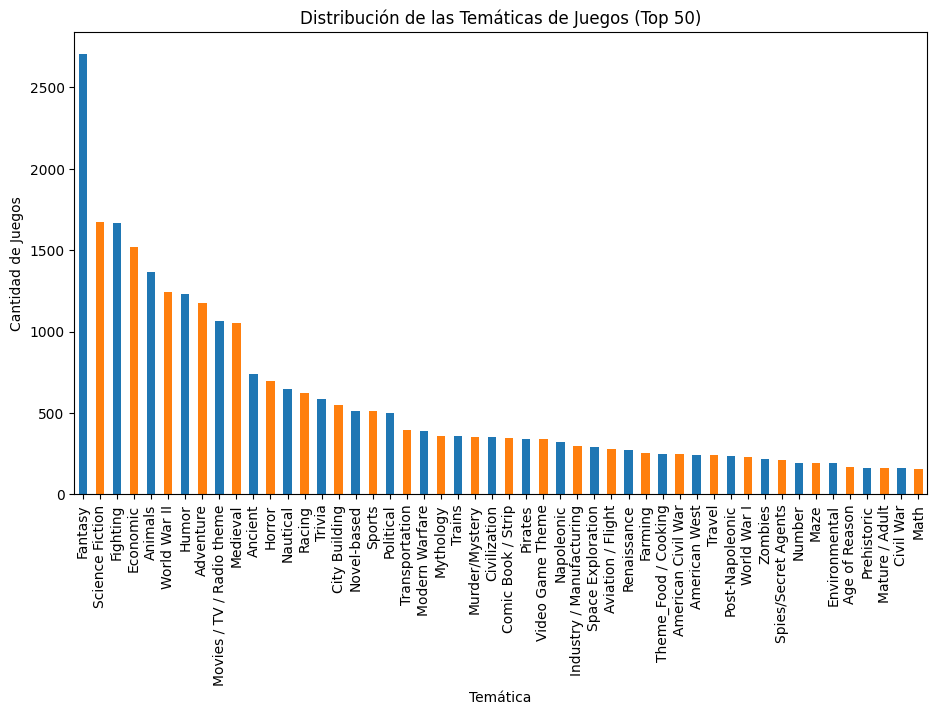
\includegraphics[width=0.8\linewidth]{tematicasComunes.png}
    \caption{Temáticas más comunes en el dataset}
    \label{fig:tematicasComunes}
\end{figure}

\begin{figure}[h]
    \centering
    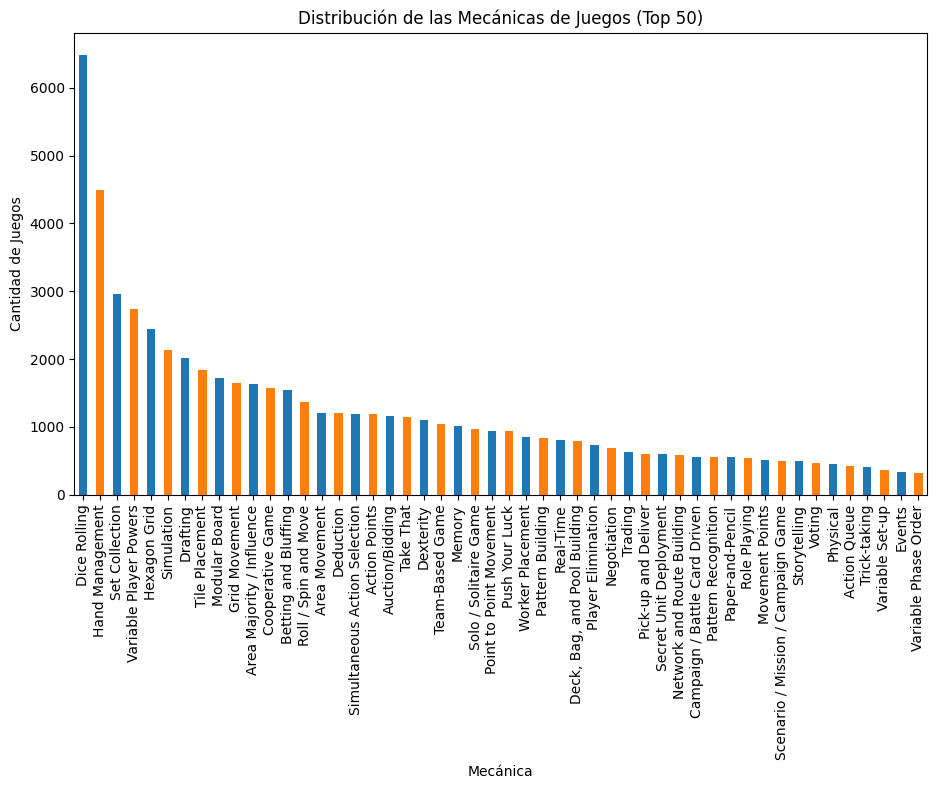
\includegraphics[width=0.8\linewidth]{mecanicasComunes.png}
    \caption{Mecánicas más comunes en el dataset}
    \label{fig:mecanicasComunes}
\end{figure}

\end{comment}

\section{Problemas identificados durante el proceso} 

Previo al pivoteo, los principales problemas que enfrentamos fueron la falta de recursos computacionales para entrenar modelos de recomendación que utilizan imágenes y la falta de experiencia en el manejo de datos de imágenes. % Creo que teníamos un problema más pero no me acuerdo cuál era.

Luego del pivoteo, los problemas que enfrentamos fueron:
\begin{itemize}
    \item Falta de obtención de metricas para comparar modelos que usan metadata.
    \item Poca flexibilidad de los modelos que utilizan metadata para recibir diferentes formatos de entrada.
\end{itemize}

\section{Revisión del plan propuesto en la etapa anterior y justificación de ajustes} 

En general, el pivoteo fue\dots %Qué tal nos fue con el pivoteo?

Para la próxima entrega, planeamos hacer que cada usuario pueda elegir que cada una de las metadatas que le corresponden tenga un peso distinto en la recomendación. Esto lo haremos \dots %Dejar alguna idea de cómo lo haremos escrita.

\section{Anexo: actualización de propuesta}
\begin{itemize}
    \item Deben agregar unos 3 baselines de métodos para recomendar grupos
    \item Deben actualizar la metodología de evaluación indicando métricas especificas para recomendación a grupos, no pueden hacer la misma evaluación que recomendar a individuos
\end{itemize}

\end{document}


